\subsection{Motherboard}

Una vegada escollits dos processadors com a contrinicants per al nostre clúster, hem mirat quines motherboards hi havia al mercat. Primerament les hem buscat de manera individual i hem seleccionat les següents.\\

% Please add the following required packages to your document preamble:
% \usepackage[table,xcdraw]{xcolor}
% If you use beamer only pass "xcolor=table" option, i.e. \documentclass[xcolor=table]{beamer}
\begin{table}[h!]
\begin{tabular}{|l|l|l|l|l|l|l|}
\hline
\rowcolor[HTML]{C0C0C0} 
Nom & \begin{tabular}[c]{@{}l@{}}Max \\ Cores\end{tabular} & \begin{tabular}[c]{@{}l@{}}Storage\\ Speed\end{tabular} & \begin{tabular}[c]{@{}l@{}}Max\\ DIMS\end{tabular} & \begin{tabular}[c]{@{}l@{}}USB\\  3.0\end{tabular} & PCI-E & Preu \\ \hline
H12DSU-iN \cite{mother1} & 64 & 6 Gbps & 32 & 5 & 1x16, 1x32, 1x40 & Coming soon \\ \hline
H12DST-B \cite{mother2} & 64 & 6 Gbps & 16 & 2 & 3x16, 1x24 & - \\ \hline
H12SSW-NT \cite{mother3} & 64 & 6 Gbps & 8 & 7 & 1x16, 1x32 & 1356.53\euro \cite{mother3_preu}\\ \hline
H12SSW-iN \cite{mother4} & 64 & 6 Gbps & 8 & 7 & 2x32 & - \\ \hline
H12SST-PS \cite{mother5} & 64 & 6 Gbps & 8 & 2 & 3x16 & 3959.86\euro \cite{mother5_preu}\\ \hline
\end{tabular}
\caption{Comparació inicial de motherboards}
\end{table}



Veiem que les diferències principals son el número de DIMS de memòria i els PCI-Express. No obstant, una vegada totes comparades, ens hem trobat amb que d'algunes no trobàvem el preu enlloc. Els llocs on trobàvem els preus no és el mateix que d'on trobavem les especificacions, per tant no estem segurs de que els preus siguin els correctes.\\

Buscant els preus ens hem trobat amb una altra web \cite{webnodes} que ens deixa crear un node seleccionant nosaltres els seus components. Hem vist que els tipus de node es diferencien inicialment entre aquells amb GPU i aquells sense GPU. Dins d'aquests dos grups, trobem també els dual-socket i els single-socket.\\

\begin{figure}[h]
    \centering
    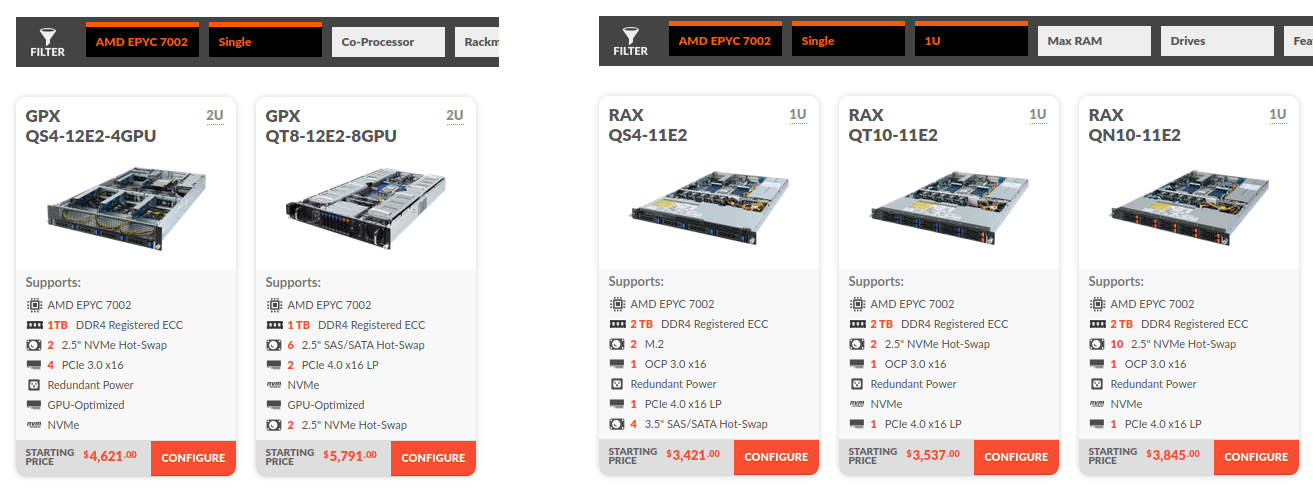
\includegraphics[width=\textwidth]{img/webnodes.png}
    \caption{Exemple de nodes que podem trobar a la web. A l'esquerra amb GPUs i a la dreta sense. Tots single-socket.}
\end{figure}

Com el processador \textit{AMD EPYC 7702P} té 64 cores i el \textit{AMD EPYC Rome 7502P} en té 32, hem decidit plantejar-nos les opcions de nodes dual-socket amb dos processadors 7502P i nodes single-socket amb el processador 7702P. En cas d'escollir un node amb suport per GPU, s'coupen dues \textit{U}s en compte de una sola. En el cas dels nodes amb dual-socket, es poden suportar fins a 8 GPUs mentres que amb els single-socket només la meitat, 4.

 En la següent taula es veuen aquestes posibles combinacions. En el cas d'utilitzar un node amb GPUs no s'ha inclos el preu de la pròpia GPU ja que això dependrà de quina escollim més endevant. Per la mateixa raó, tampoc s'ha exposat els GFLOPs de les versions amb GPU. En aquests preus tampoc s'inclouen els costos de les memòries i les targetes de xarxa.

\begin{table}[h!]
\begin{tabular}{|c|c|c|c|c|c|c|}
\hline
\rowcolor[HTML]{C0C0C0} 
\multicolumn{1}{|l|}{\cellcolor[HTML]{C0C0C0}Configuració} & \multicolumn{1}{l|}{\cellcolor[HTML]{C0C0C0}\#cores} & \multicolumn{1}{l|}{\cellcolor[HTML]{C0C0C0}\begin{tabular}[c]{@{}l@{}}GFLOPs\\  CPU\end{tabular}} & \multicolumn{1}{l|}{\cellcolor[HTML]{C0C0C0}\#GPUs} & \multicolumn{1}{l|}{\cellcolor[HTML]{C0C0C0}Us} & \multicolumn{1}{l|}{\cellcolor[HTML]{C0C0C0}Preu} & \multicolumn{1}{l|}{\cellcolor[HTML]{C0C0C0}GFLOPS/\euro} \\ \hline
\cellcolor[HTML]{EFEFEF} &  &  & - & 1 & 10001 & 0.256 \\ \cline{4-7} 
\multirow{-2}{*}{\cellcolor[HTML]{EFEFEF}\begin{tabular}[c]{@{}c@{}}Dual amb AMD\\ EPYC Rome 7502P\end{tabular}} & \multirow{-2}{*}{128} & \multirow{-2}{*}{2560} & 8 & 2 & 12266 & - \\ \hline
\cellcolor[HTML]{EFEFEF} &  &  & - & 1 & 8172 & 0.251 \\ \cline{4-7} 
\multirow{-2}{*}{\cellcolor[HTML]{EFEFEF}\begin{tabular}[c]{@{}c@{}}Single amb AMB\\ EPYC 7702P\end{tabular}} & \multirow{-2}{*}{128} & \multirow{-2}{*}{2048} & 4 & 2 & 9461 & - \\ \hline
\end{tabular}
\caption{Comparació entre les diferents configuracions dels nodes}
\end{table}


Veiem que tot i que la versió amb dual socket ens proporciona més GFLOPs, l'eficiència GFlops/\euro és millor per la versió amb single socket. Per tant, en aquest punt encara no podem decantar-nos per cap de les dues. Una vegada haguem considerat quines GPUS utilitzem, quina xarxa tenim, etc. podrem valorar si tenim suficient presupost com per escollir la opció amb més GFLOPS. Alhora, quan les GPUs entrin en joc també s'haurà de tenir en compte que amb la opció dual-socket en podem possar el doble per cada node.

